\chapter{Etica - Introduzione}

\section{Il Corso in Breve...}

Il corso ha un aspetto prettamente \fancyglitter{umanistico} e \fancyglitter{interdisciplinare}. Si andranno ad affrontare diverse prospettive che impattano su diverse dimensioni della propria vita:

\begin{itemize}
  \item Innovazione (brevetti). 
  \item Economia (monopoli). 
  \item Politica. 
  \item Giuridica. 
  \item Tecnologica.
  \item Mercato dell'attenzione.
  \item Retorica.
\end{itemize}

\dfn{Retorica}{
  L'arte del dialogare per convincere le persone a fare quello che si vuole.
}

\nt{Nei giornali, nella politica, nella pubblicità\footnote{Per questo esistono gli AdsBlocker.}, etc.}

\ex{Retorica}{
\begin{itemize}
  \item La cimice asiatica sostituirà la cimice verde nei nostri prati. 
  \item I robot sostituiranno gli esseri umani nei posti di lavoro.
\end{itemize}

Due frasi grammaticalmente identiche, ma non sono la stessa cosa: la prima ha un significato letterale, la seconda no. Perché la seconda non intende che i robot andranno a prendere e buttare via gli esseri umani dal posto di lavoro, ma che i padroni sostituiranno i lavoratori con dei robot.

Questa è una frase strumentale, per nascondere il ruolo dell'essere umano. 
}

\nt{Qualsiasi affermazione di una società è puramente strumentale. Punta a manipolare le persone per ottenere un ritorno economico.}

\subsection{Perché Questo Corso?}

\paragraph{Le tre missioni dell'università:}

\begin{itemize}
  \item Didattica. 
  \item Ricerca. 
  \item Terza missione: esportare le conoscenze tecnologiche alle aziende\footnote{Che spreco...} e rendere coscenti le persone di quello di cui si occupa l'università (opportunità e rischi).
\end{itemize}

\paragraph{I messaggi del corso:}

\begin{itemize}
  \item La tecnologia e l’impatto che ha nella società sono costruzioni sociali,
senza nessuna inevitabilità. 
\item La tecnologia non può risolvere i problemi che crea (e. g. i bias)\footnote{Fuck Silicon Valley and fuck Marc Andreessen.}. 
\item L'AI non è solo una tecnologia. 
\item L'essere umano ha un ruolo importante nel determinare l’impatto delle
tecnologie digitali, sia nella propria professione sia come
cittadini.
\end{itemize}

\paragraph{Che cosa vuol dire che l'AI non è solo una tecnologia?}

\begin{figure}[h]
    \centering
    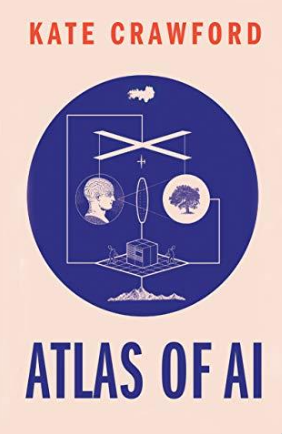
\includegraphics[scale=0.55]{01E/aoa.png}
    \caption{Uno dei libri possibili per l'esame.}
\end{figure}

\begin{itemize}
  \item In "Atlas of AI", Kate Crawford, propone un esperimento. 
  \item Prendete Google Search (schifezza) e scrivete ARTIFICIAL INTELLIGENCE. 
  \item I risultati sono immagini, principalmente di cervelli, con sfondo blu. 
  \item Cos'è che non viene mostrato? 
    \begin{itemize}
      \item L'inquinamento delle miniere di litio (con cui sono fatte le batterie). 
      \item Le proteste delle popolazioni la cui vita è stata distrutta dalle miniere di litio. 
      \item Le terre rare (metalli che servono per i microprocessori) che vengono estratte in paesi sottosviluppati, zone di guerra, da minori (spesso in cina). 
      \item Le condizioni di schiavitù in cui lavorano centinaia di persone allo sviluppo dei dispositivi elettronici.
      \item Gli enormi datacenter alimentati da fonti non rinnovabili.
      \item Per allenare i sistemi di AI vengono usate foto su cui non si hanno i diritti.
      \item The cleaners: la gente, sottopagata, che si occupa di pulire tutto lo schifo umano (decapitazioni, pedopornografia, violenza su donne, uomini, bambini, animali, etc.) in modo che i modelli di ML e i Social Media siano puliti.
      \item L'ossessione per la produttività a cui sono soggetti i lavoratori (dal Taylorismo in avanti).
      \item In alcuni paesi il riconoscimento facciale è usato per discriminare minoranze.
      \item Le varie challenge su TikTok che procurano morti. 
      \item Molly Russsel: ragazzina di 14 anni che si è suicidata dopo che Instagram e YouTube, con algoritmi AI di personalizzazione, le hanno mostrato più di 2000 contenuti di istigazione al suicidio e all'autolesionismo. 
      \item FaceBook è stato accusato di genocidio in Etiopia, Bangladesh e Myanmar per persecuzioni di minoranze. 
      \item Assalto a Capitol Hill da parte dei sostenitori di Trump, anche a causa dei Social Media. 
\begin{figure}[h]
    \centering
    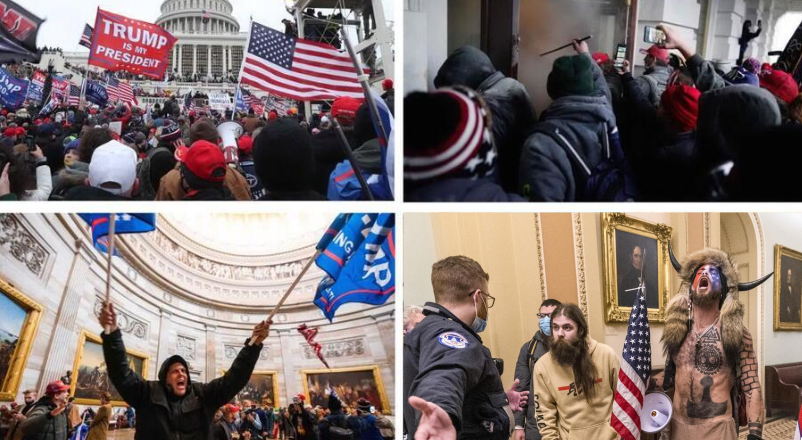
\includegraphics[scale=0.4]{01E/Trump.png}
    \caption{Assalto a Capitol Hill (6 Gennaio 2021).}
\end{figure}
\item QAnon nasce su 4chan: teoria secondo la quale il "deep state" sia composto da pedofili che rubano i bambini per estrarne il loro sangue e produrre una droga contro l'invecchiamento.
  \begin{figure}[h]
    \centering
    
\includegraphics[scale=0.25]{01E/4chan.jpg}
    \caption{Elon moment.}
\end{figure}
\item "You have blood on your hands" disse il senatore Graham a Mark Zuckenberg, "You have a product that's killing people.". 
    \end{itemize}
\end{itemize}

\paragraph{Social Network vs. Social Media:}

\begin{itemize}
  \item Un Social Network serve per mettere in connessione le persone. 
  \item Un Social Media serve per distribuire contenuti. 
  \item Diversi Social Network sono diventati Social Media (e. g. FaceBook).
\end{itemize}

\qs{}{Perché si è andati in questa direzione?}

\paragraph{Risposta:} ultimamente si mostrano i contenuti più virali, ritenuti interessanti al singolo, per creare dipendenza e aumentare gli introiti dovuti alla pubblicità. "If you're not paying for it, you're not the customer; you're the product being sold".









